\section{Datasets and Experimental results analysis} \label{section4}
this experiment uses traffic accident detection dataset which is there on hugging face \textbackslash{}cite\{hiennguyen2024accident\} there are some public datasets which provide images, object annotations, image dimensions and image-level accident flags but they never provide directly CRT targets, TTC values or intervention levels so the preprocessing pipeline is derived from these datasets in our experiments we used 3,000 scenes for training and 600 for validation then we used 120 validation scenes for the ablation study and PIKV analysis these are the splits we used in our experiments rather than separate official train and validation splits provided by the dataset Table\~\ref\{table\_datasets\} summarises them


\begin{table}[H]
\caption{Data used in our experiments.}
\centering
\label{table_datasets}
\adjustbox{max width=\linewidth}{
\begin{tabular}{l|c|c|l|l}
\hline
\textbf{Data} & \textbf{Split} & \textbf{Samples} & \textbf{Used For} & \textbf{Labels} \\
\hline
Traffic accident detection \cite{hiennguyen2024accident} & Train (our split) & 3,000 scenes & Training (5 epochs) & Derived CRT target, level (0--4) \\
Traffic accident detection \cite{hiennguyen2024accident} & Validation (our split) & 600 scenes & Model selection & Derived CRT target, level (0--4) \\
Traffic accident detection \cite{hiennguyen2024accident} & Validation subset & 120 (40 quick) & Ablation, PIKV pruning & Derived anomaly label if CRT$^{*} > 0.4$ \\
Scripted demo scenarios A--D & -- & 4 scenarios & Behaviour check & Expected level \\
\hline
\end{tabular}
}
\end{table}

\textbf{Setup.} for this experiment we used PyTorch 2.6.0 and CUDA 12.4 on Intel i7-12700H system with 16~GB RAM and NVIDIA RTX 3050 Laptop GPU (4~GB VRAM) we used AdamW with learning rate of $3 \times 10^{-4}$ and batch size 16 and when CRT is more than 0.4 we labelled that sample as anomaly for TTC-only baseline we used threshold $\min_i \text{TTC}_i < 3$~s we also set some limits for vehicle like $\mu g=6.867$~m/s$^2$, $a_{\text{lat,max}}=6.0$~m/s$^2$, and $\dot{\psi}_{\max}=1.2$~rad/s we used 30~FPS as reference and kept 10~ms as target time for each frame these values are chosen by us for this experiment they are not directly taken from the dataset

\textbf{Training behaviour.} this Figure~\ref{fig_training} shows loss and CRT MAE for five epochs validation loss reached 0.0396 and CRT MAE reached 0.0417 the training log shows 100\% validation accuracy from the first epoch but the available notes do not say if this was checked on all 600 validation scenes or only the 120 scenes we used to test different parts of the model so we did not use this figure alone to say that the model will work well on other data the difference between accident and normal scenes in those 120 scenes is discussed below

\begin{figure}[H]
\centering
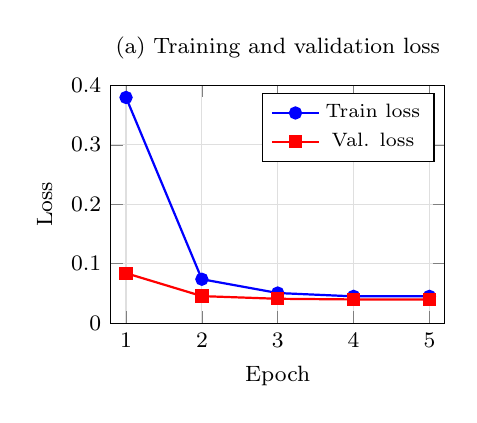
\begin{tikzpicture}
\begin{axis}[
    width=0.48\linewidth, height=4.6cm,
    xlabel={Epoch}, ylabel={Loss},
    xmin=0.8, xmax=5.2, ymin=0, ymax=0.4, xtick={1,2,3,4,5},
    grid=major, grid style={gray!25},
    legend style={font=\scriptsize}, legend pos=north east,
    tick label style={font=\footnotesize}, label style={font=\footnotesize},
    title={\footnotesize (a) Training and validation loss}]
\addplot[thick, blue, mark=*] coordinates {(1,0.3797) (2,0.0738) (3,0.0506) (4,0.0450) (5,0.0450)};
\addlegendentry{Train loss}
\addplot[thick, red, mark=square*] coordinates {(1,0.0840) (2,0.0454) (3,0.0409) (4,0.0398) (5,0.0396)};
\addlegendentry{Val. loss}
\end{axis}
\end{tikzpicture}
\hfill
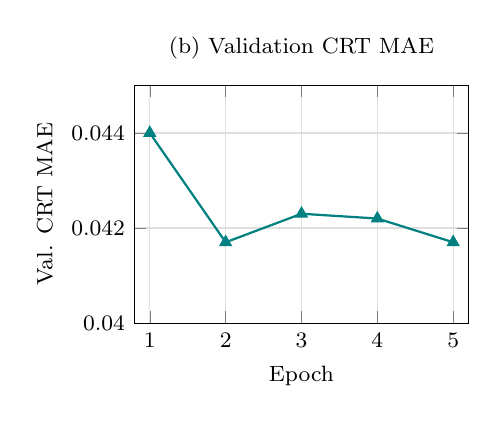
\begin{tikzpicture}
\begin{axis}[
    width=0.48\linewidth, height=4.6cm,
    xlabel={Epoch}, ylabel={Val. CRT MAE},
    xmin=0.8, xmax=5.2, ymin=0.040, ymax=0.045, xtick={1,2,3,4,5},
    yticklabel style={/pgf/number format/fixed, /pgf/number format/precision=3},
    scaled y ticks=false,
    grid=major, grid style={gray!25},
    tick label style={font=\footnotesize}, label style={font=\footnotesize},
    title={\footnotesize (b) Validation CRT MAE}]
\addplot[thick, teal, mark=triangle*] coordinates {(1,0.0440) (2,0.0417) (3,0.0423) (4,0.0422) (5,0.0417)};
\end{axis}
\end{tikzpicture}
\captionsetup{singlelinecheck = false, format= hang, justification=justified, font=footnotesize, labelsep=space}
\caption{Training history of PC-CSG on the traffic accident detection dataset \cite{hiennguyen2024accident} (3,000 training / 600 validation scenes, AdamW, learning rate $3 \times 10^{-4}$, batch size 16).}
\label{fig_training}
\end{figure}

\subsection{Hardware Profiling and Latency Breakdown}
We profiled pipeline on an RTX 3050 Laptop GPU using 10 agents, 6 counterfactuals, and 15 horizon steps. Table~ named \ref{table_latency} and Figure~named\ref{fig_latency} report  measured times.  this configuration, the pipeline reached 149.7~FPS.  hidden dimension $D=128$,  CSGA forward pass took 1.57~ms. measurement are not made on an embedded automative platform,so laptop result will not be read as embedded-device benchmark. 
\begin{table}[H]
\caption{Measured component-level inference latency on  NVIDIA RTX 3050 Laptop GPU ($N=10$ agents, $K=6$ counterfactuals, $H=15$ horizon).}
\centering
\label{table_latency}
\begin{tabular}{l|c|c}
\hline
\textbf{Pipeline Component} & \textbf{Latency (ms)} & \textbf{Share (\%)} \\
\hline
Scene Graph Construction \& Hazard Scoring & 0.33~ms & 4.9\% \\
Counterfactual Scene Graph Attention (CSGA) & 1.57~ms & 23.5\% \\
Kinematic Bicycle Model Propagation ($N \times K$) & 4.12~ms & 61.7\% \\
Physics-Informed Kinematic Validator (PIKV) & 0.53~ms & 7.9\% \\
CRT Engine \& Intervention Arbiter & 0.13~ms & 1.9\% \\
\hline
\textbf{Total PC-CSG Pipeline Latency} & \textbf{6.68~ms} & \textbf{100.0\%} \\
\textbf{Effective Real-Time Throughput} & \multicolumn{2}{c}{\textbf{149.7 FPS}} \\
\textbf{Throughput vs. 30 FPS reference target} & \multicolumn{2}{c}{\textbf{4.99$\times$ Real-Time Throughput}} \\
\hline
\end{tabular}
\end{table}

\begin{figure}[H]
\centering
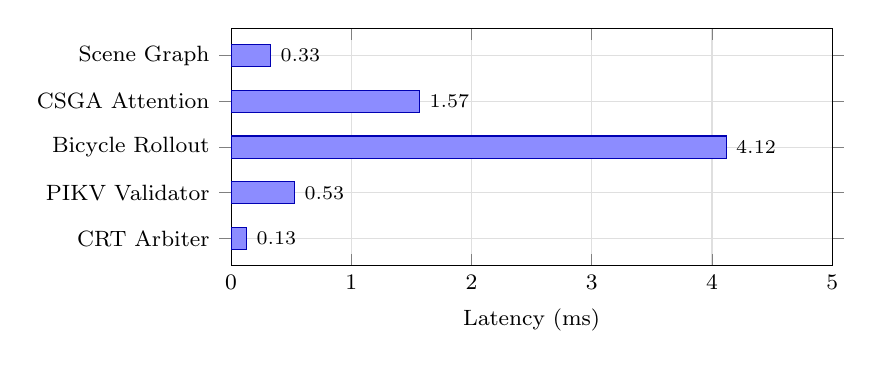
\begin{tikzpicture}
\begin{axis}[
    xbar, width=0.76\linewidth, height=4.6cm,
    xlabel={Latency (ms)}, xmin=0, xmax=5,
    ytick={1,2,3,4,5},
    yticklabels={CRT Arbiter, PIKV Validator, Bicycle Rollout, CSGA Attention, Scene Graph},
    y dir=normal, bar width=8pt, enlarge y limits=0.15,
    nodes near coords, nodes near coords align={horizontal},
    every node near coord/.append style={font=\scriptsize},
    tick label style={font=\footnotesize}, label style={font=\footnotesize},
    grid=major, grid style={gray!25}]
\addplot[fill=blue!45, draw=blue!70!black] coordinates {(0.13,1) (0.53,2) (4.12,3) (1.57,4) (0.33,5)};
\end{axis}
\end{tikzpicture}
\captionsetup{singlelinecheck = false, format= hang, justification=justified, font=footnotesize, labelsep=space}
\caption{Component-level latency of PC-CSG on an NVIDIA RTX 3050 Laptop GPU (total 6.68~ms, 149.7~FPS).}
\label{fig_latency}
\end{figure}

measured end-to-end latency was 6.68~ms, equivalent to 149.7~FPS.  above the 30~FPS reference target and below separate 10~ms per-frame design target. The bicycle rollout took 4.12~ms (61.7\% of the total), while CSGA took 1.57~ms. A Python loop launches small GPU kernels over  15 rollout steps and contributes to the cost;  combining these operations with \texttt{torch}.overhead may be reduced by compile, but that improvement has not yet  measured.

\subsection{PIKV Validation Effectiveness}
120 validation scenes contained 113 critical vehicles, from which the system generated 678 counterfactual hypotheses. PIKV filtered out 312 hypotheses (\textbf{46.0\%}) in total. The results for each mode appear in Table~named \ref{table_pruning} and Figurename~\ref{fig_pikv}.

\begin{table}[H]
\caption{PIKV hypothesis pruning across the six counterfactual modes (678 hypotheses, 113 per mode, from real traffic validation samples).}
\label{table_pruning}
\centering
\adjustbox{max width=\linewidth}{
\begin{tabular}{l|c|l}
\hline
\textbf{Counterfactual Mode} & \textbf{Pruning Rate} & \textbf{Main Rejection Reason} \\
\hline
\texttt{sudden\_brake} & 0.0\% & Straight-line deceleration stays inside the friction circle \\
\texttt{hard\_swerve\_left} & 70.8\% & Lateral acceleration exceeds $a_{\text{lat,max}}$ / friction circle \\
\texttt{hard\_swerve\_right} & 21.2\% & Rejected only when path curvature breaks friction limits \\
\texttt{sudden\_acceleration} & 100.0\% & Surge combined with learned steering breaks $a_{\text{total}} \le \mu g$ \\
\texttt{lane\_departure} & 73.5\% & Yaw rate exceeds $\dot{\psi}_{\max} = 1.2$~rad/s \\
\texttt{stationary\_obstacle} & 10.6\% & Feasible unless stopping needs more than the available deceleration \\
\hline
\textbf{Overall Pruning Rate} & \textbf{46.0\%} & \textbf{312 / 678 hypotheses filtered} \\
\hline
\end{tabular}
}
\end{table}

\begin{figure}[H]
\centering
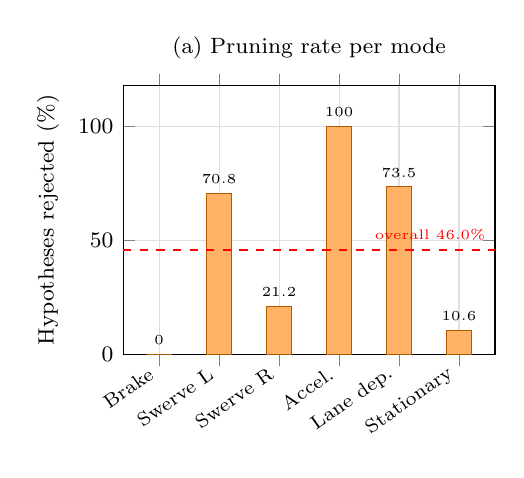
\begin{tikzpicture}
\begin{axis}[
    ybar, width=0.52\linewidth, height=5.0cm,
    ylabel={Hypotheses rejected (\%)}, ymin=0, ymax=118,
    xtick={1,2,3,4,5,6},
    xticklabels={Brake, Swerve L, Swerve R, Accel., Lane dep., Stationary},
    x tick label style={rotate=35, anchor=east, font=\scriptsize},
    xmin=0.4, xmax=6.6, bar width=9pt,
    nodes near coords, every node near coord/.append style={font=\tiny},
    tick label style={font=\footnotesize}, label style={font=\footnotesize},
    grid=major, grid style={gray!25},
    title={\footnotesize (a) Pruning rate per mode}]
\addplot[fill=orange!60, draw=orange!70!black] coordinates {(1,0.0) (2,70.8) (3,21.2) (4,100.0) (5,73.5) (6,10.6)};
\draw[dashed, red, thick] (axis cs:0.4,46.0) -- (axis cs:6.6,46.0);
\node[font=\tiny, red, anchor=south east] at (axis cs:6.6,46.0) {overall 46.0\%};
\end{axis}
\end{tikzpicture}
\hfill
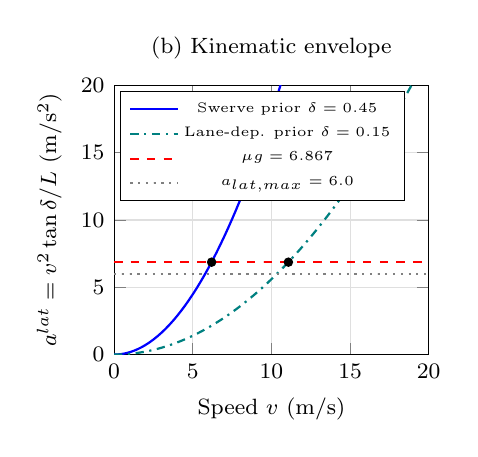
\begin{tikzpicture}
\begin{axis}[
    width=0.46\linewidth, height=5.0cm,
    xlabel={Speed $v$ (m/s)}, ylabel={$a^{\text{lat}} = v^2 \tan\delta / L$ (m/s$^2$)},
    xmin=0, xmax=20, ymin=0, ymax=20, domain=0:20, samples=81,
    restrict y to domain=0:25,
    legend style={font=\tiny, at={(0.02,0.98)}, anchor=north west},
    tick label style={font=\footnotesize}, label style={font=\footnotesize},
    grid=major, grid style={gray!25},
    title={\footnotesize (b) Kinematic envelope}]
\addplot[thick, blue] {x^2*0.48306/2.7};
\addlegendentry{Swerve prior $\delta = 0.45$}
\addplot[thick, teal, dashdotted] {x^2*0.15114/2.7};
\addlegendentry{Lane-dep. prior $\delta = 0.15$}
\addplot[thick, red, dashed, domain=0:20] {6.867};
\addlegendentry{$\mu g = 6.867$}
\addplot[thick, gray, dotted, domain=0:20] {6.0};
\addlegendentry{$a_{\text{lat,max}} = 6.0$}
\addplot[only marks, mark=*, mark size=1.5pt] coordinates {(6.20,6.867) (11.08,6.867)};
\end{axis}
\end{tikzpicture}
\captionsetup{singlelinecheck = false, format= hang, justification=justified, font=footnotesize, labelsep=space}
\caption{PIKV validation analysis: (a) pruning rate per mode; (b) lateral acceleration envelope ($L=2.7$~m).}
\label{fig_pikv}
\end{figure}

The rejection pattern depends on the kinematic limits configured for this experiment. The straight-braking prior of $-5$~m/s$^2$ stays below the configured friction limit of $6.867$~m/s$^2$, so none of those hypotheses were removed. With the sharp-swerve setting ($\delta = 0.45$), the lateral-acceleration curve crosses the same limit at about 22~km/h (6.2~m/s); this is consistent with the high rejection rate at the tested speeds. Left and right swerves still differ: PIKV rejected 70.8\% of left-swerve hypotheses and 21.2\% of right-swerve hypotheses, although their priors were symmetric. Decoder residuals or dataset bias may explain the difference. All sudden-acceleration hypotheses were rejected because the learned steering residuals pushed total acceleration above $\mu g$.

\subsection{Ablation Study and Risk Analysis}
We compared five model configurations on the 120-sample validation subset. Table~\ref{table_ablation} reports their accuracy, FPR, and per-sample latency.

\begin{table}[H]
\caption{Ablation study on the 120-sample validation split (anomaly threshold CRT $> 0.4$).}
\centering
\label{table_ablation}
\adjustbox{max width=\linewidth}{
\begin{tabular}{l|c|c|c}
\hline
\textbf{Configuration} & \textbf{Accuracy (\%)} & \textbf{FPR (\%)} & \textbf{Latency / sample (ms)} \\
\hline
Reactive TTC-Only Baseline (anomaly if $\min_i \text{TTC}_i < 3$~s) & 94.2 & 100.0 & 0.08 \\
Scene Graph Attention only (No CF, No PIKV) & 5.8 & 0.0 & 0.20 \\
CSGA without PIKV (unconstrained counterfactuals) & 100.0 & 0.0 & 0.51 \\
CSGA + PIKV without causal gate input & 100.0 & 0.0 & 0.51 \\
\textbf{PC-CSG Full (CSGA + PIKV + causal gate head)} & \textbf{100.0} & \textbf{0.0} & \textbf{0.92} \\
\hline
\end{tabular}
}
\end{table}

ablation timing not really matching with component profile in Table~\ref{table_latency} like CSGA without PIKV showing 0.51~ms but CSGA itself is 1.57~ms and PIKV 0.53~ms in component profile, so i am not sure how both are being measured because numbers are not matching like we expected  both are measuring different things or some timing procedure is different but notes are not saying anything about this. we  not just directly compare both and say this much time is taken by each component, need to check what exactly is measured first, it will be confusing when explaining results.

also 120 scene subset  having very imbalanced data,so  TTC baseline marked all samples as anomaly and got 94.2\% accuracy with 100\% FPR which looks good only when we see accuracy but actually it predicted every single one as anomaly. scene graph attention did opposite and predicted no anomaly at all so accuracy only 5.8\% and FPR 0\%. there are around 94.2\% hazard scenes and only seven benign scenes which is just 5.8\%, so obviously predicting everything as hazard will give high accuracy here. i think this is important because accuracy is not telling properly how good model is doing and we should not take it like TTC baseline is working better just because number is high. counterfactual variants got all 120 samples correct which is nice but still dataset is small and mostly one type of samples so need more balanced data also before saying results will work generally.

PIKV and FPR part also we cannot really confirm from this subset because only seven benign scenes are available, maybe it is not enough to show actual reduction in FPR from experiment. Proposition~2 says PIKV cannot increase FPR but that is different from saying we measured a reduction in FPR here, both are not same thing and i think we should not mix it up while writing results. also causal gate scores are being calculated but currently they are not multiplied into attention weights so it is not actually changing attention right now. we have scores but they are not used in a way that can change weights yet, so this ablation is not really showing any effect from causal gate and we need to keep this part in mind.

Figure~\ref{fig_scenarios} shows four scripted scenarios and in Scenarios B--D CRT follows hazard curve $H(\text{TTC})$. current gate setting says when $H \ge 0.25$ then TTC should be $\le 3.55$~s, so if TTC is more than 3.55~s Level~1 alert cannot happen with current threshold. this is coming from current threshold setting itself and not something else from results, like even if we look at scenarios and expect an alert at higher TTC it cannot happen because condition is not satisfied. so this limit is already there in current setup and probably need to think about this when discussing what CRT is doing in different scenarios.

\begin{table}[H]
\caption{Measured behaviour of PC-CSG on the four scripted demo scenarios.}
\centering
\label{table_scenarios}
\adjustbox{max width=\linewidth}{
\begin{tabular}{l|l|c|c|c|l}
\hline
\textbf{Scenario} & \textbf{Driving Context} & \textbf{Ego Speed} & \textbf{Worst TTC} & \textbf{CRT} & \textbf{Level / Action} \\
\hline
A & Highway cruise, all clear & 100.1~km/h & 33.3~s & 0.000 & Level 0: nominal cruise \\
B & Lead vehicle decelerating & 110.2~km/h & 4.1~s & 0.103 & Level 0: monitoring \\
C & Lane-change swerve conflict & 119.9~km/h & 1.9~s & 0.894 & Level 4: AEB + MRM \\
D & Barrier + hard lead braking & 100.1~km/h & 0.5~s & 0.987 & Level 4: full AEB \\
\hline
\end{tabular}
}
\end{table}

\begin{figure}[H]
\centering
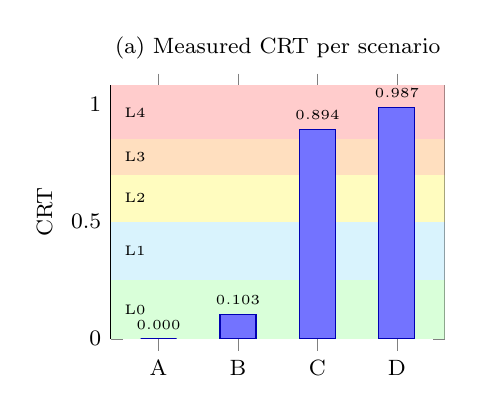
\begin{tikzpicture}
\begin{axis}[
    ybar, width=0.48\linewidth, height=4.8cm,
    ylabel={CRT}, ymin=0, ymax=1.08,
    xtick={1,2,3,4}, xticklabels={A, B, C, D},
    xmin=0.4, xmax=4.6, bar width=13pt,
    nodes near coords={\pgfmathprintnumber[fixed, fixed zerofill, precision=3]{\pgfplotspointmeta}},
    every node near coord/.append style={font=\tiny},
    tick label style={font=\footnotesize}, label style={font=\footnotesize},
    title={\footnotesize (a) Measured CRT per scenario}]
\fill[green!15] (axis cs:0.4,0) rectangle (axis cs:4.6,0.25);
\fill[cyan!15] (axis cs:0.4,0.25) rectangle (axis cs:4.6,0.50);
\fill[yellow!25] (axis cs:0.4,0.50) rectangle (axis cs:4.6,0.70);
\fill[orange!25] (axis cs:0.4,0.70) rectangle (axis cs:4.6,0.85);
\fill[red!20] (axis cs:0.4,0.85) rectangle (axis cs:4.6,1.08);
\node[font=\tiny, anchor=west] at (axis cs:0.45,0.125) {L0};
\node[font=\tiny, anchor=west] at (axis cs:0.45,0.375) {L1};
\node[font=\tiny, anchor=west] at (axis cs:0.45,0.60) {L2};
\node[font=\tiny, anchor=west] at (axis cs:0.45,0.775) {L3};
\node[font=\tiny, anchor=west] at (axis cs:0.45,0.965) {L4};
\addplot[fill=blue!55, draw=blue!70!black] coordinates {(1,0.000) (2,0.103) (3,0.894) (4,0.987)};
\end{axis}
\end{tikzpicture}
\hfill
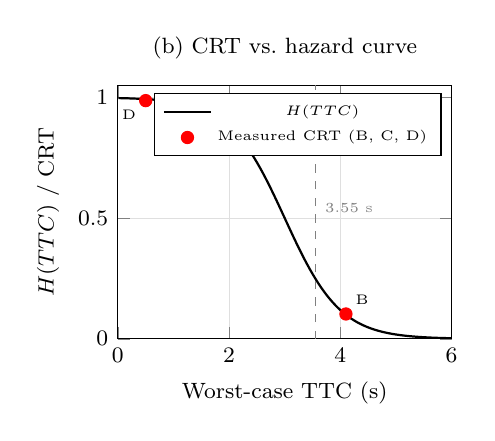
\begin{tikzpicture}
\begin{axis}[
    width=0.48\linewidth, height=4.8cm,
    xlabel={Worst-case TTC (s)}, ylabel={$H(\text{TTC})$ / CRT},
    xmin=0, xmax=6, ymin=0, ymax=1.05, domain=0.01:6, samples=121,
    legend style={font=\tiny}, legend pos=north east,
    tick label style={font=\footnotesize}, label style={font=\footnotesize},
    grid=major, grid style={gray!25},
    title={\footnotesize (b) CRT vs.\ hazard curve}]
\addplot[thick, black] {1/(1+exp((x-3.0)/0.5))};
\addlegendentry{$H(\text{TTC})$}
\addplot[only marks, mark=*, mark size=2.2pt, red] coordinates {(4.1,0.103) (1.9,0.894) (0.5,0.987)};
\addlegendentry{Measured CRT (B, C, D)}
\addplot[thin, gray, dashed] coordinates {(3.55,0) (3.55,1.05)};
\node[font=\tiny, anchor=south west] at (axis cs:4.1,0.103) {B};
\node[font=\tiny, anchor=south west] at (axis cs:1.9,0.894) {C};
\node[font=\tiny, anchor=north east] at (axis cs:0.5,0.987) {D};
\node[font=\tiny, anchor=north west, gray] at (axis cs:3.55,0.6) {3.55 s};
\end{axis}
\end{tikzpicture}
\captionsetup{singlelinecheck = false, format= hang, justification=justified, font=footnotesize, labelsep=space}
\caption{Demo scenarios: (a) CRT values and intervention bands; (b) CRT vs.\ hazard curve.}
\label{fig_scenarios}
\end{figure}

\subsection{Capability Comparison with Related Methods}
methods review here adress different task, from trajectory to offline testing. we was not evalute them on shared datase, thats why accuracy comparison may not be reliable. Table~\ref{table_comparison} instead summarises the capabilities described in the cited papers.

\begin{table}[H]
\caption{related methods compatibility comparison,  based on the descriptions in the original papers. Latency is given only for PC-CSG because  other papers do not report it on comparable hardware.}
\centering
\label{table_comparison}
\adjustbox{max width=\linewidth}{
\begin{tabular}{l|c|c|c|c|c|l}
\hline
\textbf{Method} & \textbf{Venue / Year} & \textbf{Counterfactual Hypotheses} & \textbf{Physics Check} & \textbf{Interaction Structure} & \textbf{Risk $\rightarrow$ Action} & \textbf{Setting} \\
\hline
TTC-only baseline & -- & No & No & No & Binary & Online, reactive \\
CRiTIC \cite{ahmadi2025critic} & ICRA 2025 & No & No & Causal gating & No & Online prediction \\
CICR \cite{han2025cicr} & J. Imaging 2025 & Yes (counterfactual decoder) & No & Social context & No & Pedestrian prediction \\
Liao et al. \cite{liao2024physics} & IJCAI 2024 & No & Bicycle model & Interaction encoder & No & Prediction \\
TPK \cite{baden2025tpk} & IV 2025 & No & Kinematic layer & Interaction priors & No & Prediction \\
CounterScene \cite{jing2026counterscene} & arXiv 2026 & Yes (causal agent) & No & Causal interaction graph & No & Offline testing \\
STRAP \cite{ning2025strap} & ITSC 2025 & No & No & Risk-field attention & No & Prediction \\
\hline
\textbf{PC-CSG (ours)} & -- & \textbf{Yes (6 modes)} & \textbf{PIKV (6 checks)} & \textbf{Scene graph} & \textbf{5 levels} & \textbf{Online, 6.68~ms} \\
\hline
\end{tabular}
}
\end{table}

Table~\ref{table_comparison} is comparing different methods but all of them are not really doing same thing, like CRiTIC \cite{ahmadi2025critic} is selecting relevant agents while CICR \cite{han2025cicr} is working on pedestrian trajectory prediction and also using counterfactual decoder. its front-door criterion is part of causal intervention fusion module so it is not exactly doing same thing as our method. CounterScene \cite{jing2026counterscene} also looks at counterfactual futures and Liao et al. \cite{liao2024physics} and TPK \cite{baden2025tpk} are adding constraints related to vehicle motion. so when we look at all these methods each one is covering some part of problem but among selected works we didnt identify any method combining physics checked counterfactual risk with graded driver assistance actions inside perception loop. this is where PC-CSG is trying to bring these things together instead of looking at them separately. also it processed one frame in 6.68~ms on tested laptop GPU which is another thing we measured, but still we should be careful while comparing because forecasting accuracy was not measured on common dataset and we cannot say PC-CSG is more accurate than other methods from this table. It is basically a capability comparison and not direct performance comparison across all methods. also TTC only baseline is our own reactive reference implementation using 3~s cutoff, this cutoff is just our experimental setting and not something we are claiming is used by some published method. We think this difference should be clear otherwise table might give impression that all methods were tested in same way which is not what we did.

\section{Conclusion and future scope} \label{section5}
On the RTX 3050 Laptop GPU, PC-CSG processed a frame in 6.68~ms (149.7~FPS), and PIKV rejected 312 of 678 counterfactual hypotheses (46.0\%). On the 120-sample ablation subset, PC-CSG recorded 100.0\% accuracy and 0.0\% FPR, compared with 94.2\% accuracy and 100.0\% FPR for the reactive TTC baseline. These measurements indicate that the pipeline can run within the tested laptop's timing budget, but they do not establish performance on embedded automotive hardware or generalisation to a broader data distribution. As described in the analysis, PIKV removes friction-violating hypotheses from the risk score, the physics layers are reference-frame independent, and the risk score increases as TTC decreases. Proposition~2 states that PIKV does not increase FPR.


in current implementation, several limitation remails , in this given thing validation subset is small and imbalanced and physics loss provies no gradient, also casual gate is computed but not applied to the attention weights. this TTc gate prevents a level 1 warning when this TTC exceeds 3.55s. reliable warning lead time has not measured yet. these finding points to two next steps
\begin{enumerate}
    \item \textbf{Multi-modal counterfactual fusion:} this does not test what happen when camera information is unavilable. Extending CSGA to use camera, LiDAR, and radar tracks together, then testing on nuScenes \cite{caesar2020nuscenes} and Waymo Open \cite{sun2020waymo}, would help measure whether scores remain useful in rain, glare,low light.
    \item \textbf{V2X cooperative counterfactual graphs:} this scene is limited to agents available to vehecles own sensor. Sharing scene graphs and CRT values with nearby vehicles or roadside unit,links could ad d some information about agents hidden from sensors, for ex: vehicle behind a truck
\end{enumerate}

\bibliography{mybibfile}

\end{document}
